\documentclass[bachelor, och, labwork]{shiza}
% параметр - тип обучения - одно из значений:
%    spec     - специальность
%    bachelor - бакалавриат (по умолчанию)
%    master   - магистратура
% параметр - форма обучения - одно из значений:
%    och   - очное (по умолчанию)
%    zaoch - заочное
% параметр - тип работы - одно из значений:
%    referat    - реферат
%    coursework - курсовая работа (по умолчанию)
%    diploma    - дипломная работа
%    pract      - отчет по практике
% параметр - включение шрифта
%    times    - включение шрифта Times New Roman (если установлен)
%               по умолчанию выключен
\usepackage{subfigure}
\usepackage{tikz,pgfplots}
\pgfplotsset{compat=1.5}
\usepackage{float}
\usepackage{pdfpages}

\usepackage{titlesec}
\setcounter{secnumdepth}{4}
\titleformat{\paragraph}
{\normalfont\normalsize}{\theparagraph}{1em}{}
\titlespacing*{\paragraph}
{35.5pt}{3.25ex plus 1ex minus .2ex}{1.5ex plus .2ex}

\titleformat{\paragraph}[block]
{\hspace{1.25cm}\normalfont}
{\theparagraph}{1ex}{}
\titlespacing{\paragraph}
{0cm}{2ex plus 1ex minus .2ex}{.4ex plus.2ex}

% --------------------------------------------------------------------------%


\usepackage[T2A]{fontenc}
\usepackage[utf8]{inputenc}
\usepackage{graphicx}
\graphicspath{ {./images/} }
\usepackage{tempora}
\usepackage{kantlipsum}
\usepackage[sort,compress]{cite}
\usepackage{amsmath}
\usepackage{amssymb}
\usepackage{amsthm}
\usepackage{fancyvrb}
\usepackage{listings}
\usepackage{listingsutf8}
\usepackage{longtable}
\usepackage{array}
\usepackage[english,russian]{babel}

%\usepackage[colorlinks=true]{hyperref}
\usepackage{url}

\usepackage{underscore}
\usepackage{setspace}
\usepackage{indentfirst} 
\usepackage{mathtools}
\usepackage{amsfonts}
\usepackage{enumitem}
\usepackage{tikz}

\newcommand{\eqdef}{\stackrel {\rm def}{=}}
\newcommand{\specialcell}[2][c]{%
	\begin{tabular}[#1]{@{}c@{}}#2\end{tabular}}

\renewcommand\theFancyVerbLine{\small\arabic{FancyVerbLine}}

\begin{document}

	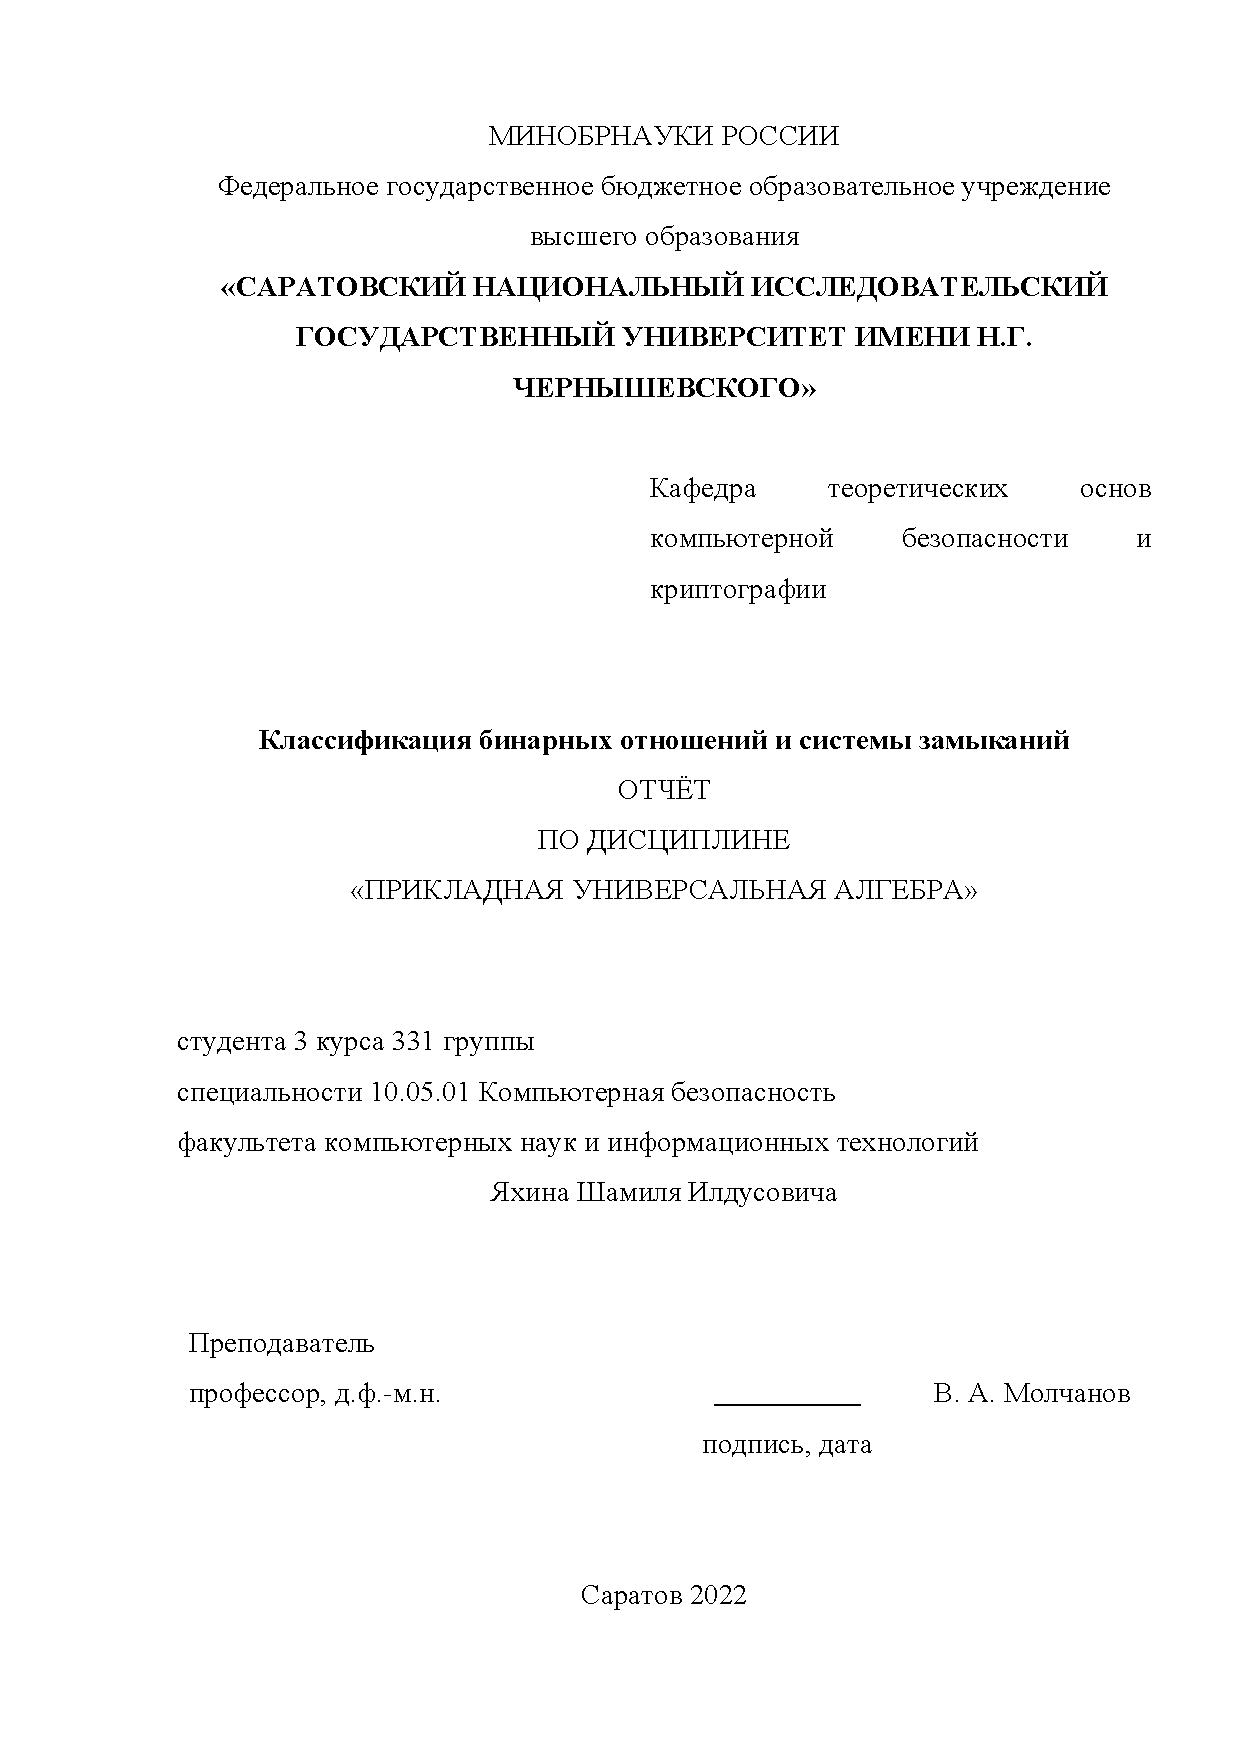
\includepdf{yahin-titulnik.pdf}
	
	%-------------------------------------------------------------------------------------------
	\tableofcontents
	
	\newpage
	
	Цель работы: изучение основных свойств бинарных отношений и операций замыкания бинарных отношений.
	
	\section{Бинарные отношения}
	    \subsection{Определение бинарного отношения}
	
	Подмножества декартова произведения $A \times B$ множеств $A$ и $B$ называются бинарными отношениями между элементами множеств $A, B$ и обозначаются строчными греческими буквами: 
	$\rho,\sigma, ..., \rho_1, \rho_2, ...   $.
	
	Для бинарного отношения $\rho \subset A \times B$ область определения $D_\rho$ и множество значений $E_\rho$ определяются как подмножества соответствующих множеств $А$ и $В$ по следующим формулам:
	
	 $D_\rho = \{a: (a,b) \in \rho $ для некоторого $ b \in B \}$,
	 
	 
	 $E_\rho = \{b: (a,b) \in \rho $ для некоторого $ a \in A \}$. 
	

    \subsection{Классификация бинарных отношений}

	Бинарное отношение $\rho \subset A \cdot A$ называется:

	\begin{enumerate}
		\item \textit{рефлексивным}, если $(a, a) \in \rho$, для любого $a \in A$;
		\item \textit{симметричным}, если $(a, b) \in \rho \Rightarrow (b, a) \in \rho$, для любого $a, b \in A$;
		\item \textit{антисимметричным}, если $(a, b) \in \rho \text{ и } (b, a) \in \rho \Rightarrow a = b$, для любых $a, b \in A$;
		\item \textit{транзитивным}, если $(a, b) \in \rho \text{ и } (b, c) \in \rho \Rightarrow (a, c) \in \rho$, для любых $a, b, c \in A$;
	\end{enumerate}
	
	Основываясь на этом, можно выделить три типа отношений:
	
	\begin{enumerate}
		\item Отношение эквивалентности
		
		Бинарное отношение $\varepsilon $ на множестве $A$ называется отношением эквивалентности (или просто $\textit{эквивалентностью}$), если оно рефлексивно, симметрично и транзитивно,
		\item Отношение квазипорядка
		
		Бинарное отношение $\omega $ на множестве $A$ называется отношением квазипорядка (или просто $\textit{квазипорядком}$), если оно рефлексивно и транзитивно,
		\item Отношение порядка
		
		Бинарное отношение $\omega $ на множестве $A$ называется отношением порядка (или просто $\textit{порядком}$), если оно рефлексивно, антисимметрично и транзитивно,
	\end{enumerate}
		
	Для того, чтобы реализовать алгоритм классификации бинарных отношений, удобно пользоваться матрицей бинарного отношения.
	
	$\textit{Матрицей}$ бинарного отношения $\rho$ между элементами множеств $A = \{a_1, ..., a_m\}$ и $B = \{b_1, ..., b_n\}$ называется прямоугольная таблица $M(\rho)$, состоящая из $m$ строк и $n$ столбцов, в которой на пересечении i-ой строки и j-го столбца стоит элемент $[M(\rho)]_{ij}$ из множества {0,1}, определяемый по правилу:
	
	\begin{equation*}
		[M(\rho)]_{ij} =  
		\begin{cases}
			1 &\text{, если $(a_i, b_j) \in \rho$}\\
			0 &\text{, в противном случае}
		\end{cases}
	\end{equation*}


		\section{Системы замыканий}
	\subsection{Определение системы замыканий}
	
	Множество Z подмножеств множества A называется $\textit{системой замыканий}$, если оно замкнуто относительно пересечений, т.е. выполняется 
	
	$\cap B \in Z $ для любого подмножества $B \subset Z $
	
	
	\subsection{Лемма о системах замыканий бинарных отношений}
	  На множестве $P(A^2)$ всех бинарных отношений между элементами множества $A$ следующие множества являются системами замыканий:
	
	\begin{enumerate}
		\item $Z_r$ - множество всех рефлексивных бинарных отношений между элементами множества $A$,
		\item $Z_s$ – множество всех симметричных бинарных отношений между элементами множества $A$,
		\item $Z_t$ – множество всех транзитивных бинарных отношений между элементами множества $A$,
		\item $Z_{eq} = Eq(A)$ – множество всех отношений эквивалентности на множестве $A$.
	\end{enumerate}

	Множество $Z_{as}$ всех антисимметричных бинарных отношений между элементами множетсва $A$ не является системой замыкания.
	
	\section{Результаты работы}
	\subsection{Описание алгоритма классификации бинарных отношений}
	
	Из пункта 1.2 следует, что в нашем алгоритме будут определяться 5 свойств бинарных отношений, а именно:
	
	\begin{enumerate}
		\item рефлексивность,
		\item антирефлексивность,
		\item симметричность,
		\item антисимметричность,
		\item транзитивность.
	\end{enumerate}
	
		Как по матрице представления определить свойства бинарного отношения:
	\begin{enumerate}
		\item Для того, чтобы бинарное отношение было $\textit{рефлексивным}$, на главной  диагонали должны стоять только единицы,
		\item Для того, чтобы бинарное отношение было $\textit{антирефлексивным}$, на главной  диагонали должны стоять только нули,
		\item Для того, чтобы бинарное отношение было $\textit{симметричным}$, матрица представления должна равняться транспонированной матрице,
		\item Для того, чтобы бинарное отношение было $\textit{антисимметричным}$, в матрице должны отсутствовать единицы, симметричные относительно главной диагонали,
		\item Для того, чтобы бинарное отношение было $\textit{транзитивным}$, матрица, полученная перемножением матрицы саму на себя, должна являться частью исходной матрицы бинарного отношения.

	\end{enumerate}
				
	Распишем алгоритмы проверки этих свойств:
	
	\subsubsection{Алгоритм проверки рефлексивности}
	
	$\textit{Вход:}$ Размерность матрицы N и матрица представления бинарного отношения размерности $N \times N$
	
	$\textit{Выход:}$  "Бинарное отношение является рефлексивным" или "Бинарное отношение не является рефлексивным".
	
	\underline{Шаг 1.} res := 0;
	
	\underline{Шаг 2.} Цикл $for$ i от 1 до N;
	
	\underline{Шаг 3.} Если a[i][i] = 1, то res := 1. Иначе res := 0;
	
	\underline{Шаг 4.} Если res = 0, то вернуть ответ "отношение не рефлексивно". Если res = 1, то вернуть ответ "отношение рефлексивно".
	
	Временная сложность алгоритма определения рефлексивности = $O(n)$
	
	\subsubsection{Алгоритм проверки антирефлексивности}

	$\textit{Вход:}$ Размерность матрицы N и матрица представления бинарного отношения размерности $N \times N$
	
	$\textit{Выход:}$  "Бинарное отношение является антирефлексивным" или "Бинарное отношение не является антирефлексивным".
	
	\underline{Шаг 1.} res := 0;

	\underline{Шаг 2.} Цикл $for$ i от 1 до N;
	
	\underline{Шаг 3.} Если a[i][i] = 0, то res := 1. Иначе res := 0;
	
	\underline{Шаг 4.} Если res = 0, то вернуть ответ "отношение не антирефлексивно". Если res = 1, то вернуть ответ "отношение антирефлексивно".
	
	Временная сложность алгоритма определения антирефлексивности = $O(n)$
		
	\subsubsection{Алгоритм проверки симметричности}
	
	$\textit{Вход:}$ Размерность матрицы N и матрица представления бинарного отношения размерности $N \times N$
	
	$\textit{Выход:}$ "Бинарное отношение является симметричным" или "Бинарное отношение не является симметричным".
	
	\underline{Шаг 1.} res := 0;
	
	\underline{Шаг 2.} Цикл $for$ i от 1 до N и в нем еще один цикл от с j от i+1 до N;
	
	\underline{Шаг 3.} Если a[i][j] = a[i][j], то res := 1. Иначе res := 0;
	
	\underline{Шаг 4.} Если res = 1, то вернуть ответ "отношение симметрично". Если res = 0, то вернуть ответ "отношение не симметрично".
	
	Временная сложность алгоритма определения симметричности = $O(n^2/2)$ = $O(n^2)$
	
	\subsubsection{Алгоритм проверки антисимметричности}
	
	$\textit{Вход:}$ Размерность матрицы N и матрица представления бинарного отношения размерности $N \times N$
	
	$\textit{Выход:}$  "Бинарное отношение является антисимметричным" или "Бинарное отношение не является антисимметричным".
	
	\underline{Шаг 1.} res := 0;

	\underline{Шаг 2.} Цикл $for$ i от 1 до N и в нем еще один цикл от с j от i+1 до N;
	
	\underline{Шаг 3.} Если  a[i][j] = a[j][i] = 1, то проверяется равенство i = j и если элементы равны, то res := 1. Иначе res = 0. Если элементы не равны единице, то res := 1;
	
	\underline{Шаг 4.} Если res = 1, то вернуть ответ "отношение антисимметрично". Если res = 0, то вернуть ответ "отношение не антисимметрично".
	
	Временная сложность алгоритма определения антисимметричности = $O(n^2/2)$ = $O(n^2)$
	
	\subsubsection{Алгоритм проверки транзитивности}

	$\textit{Вход:}$ Размерность матрицы N и матрица представления бинарного отношения размерности $N \times N$
	
	$\textit{Выход:}$  "Бинарное отношение является транзитивным" или "Бинарное отношение не является транзитивным".
	
	\underline{Шаг 1.} res := 0;
	
	\underline{Шаг 2.} Цикл $for$ i от 1 до N и в нем еще один цикл от с j от 0 до N и в нем еще один цикл с k от 0 до N;
	
	\underline{Шаг 3.} Если  a[i][k] * a[k][j] <= a[i][j], то res := 1. Иначе res := 0;
	
	\underline{Шаг 4.} Если res = 1, то вернуть ответ "отношение транзитивно". Если res = 0, то вернуть ответ "отношение не транзитивно".
	
	После проверки бинарного отношения на эти 5 свойств, мы можем судить, к какому типу отношений относится данное бинарное отношение. В этом  и заключается алгоритм классификации. Эти проверки проводятся в функции $bo\_result$.
	
	Временная сложность алгоритма определения транзитивности = $O(n^3)$
		
	\begin{enumerate}
		\item Бинарное отношение является отношением эквивалентности, если выполнились следующие три свойства: рефлексивность, симметричность и транзитивность.
		\item Если выполнились свойства рефлексивности и транзитивности, то это отношение является отношением квазипорядка,
		\item Бинарное отношение является отношением порядка, если оно рефлексивно, антисимметрично и транзитивно.
	\end{enumerate}	

	\subsubsection{Алгоритм проверки отношения на эквивалентность, квазипорядок и порядок}
	

	$\textit{Вход:}$ Размерность матрицы N и матрица представления бинарного отношения размерности $N \times N$
	
	$\textit{Выход:}$ <<Данное отношение является отношением эквивалентности>> или <<Данное отношение является отношением квазипорядка>> или <<Данное отношение является отношением порядка>>.
	
	\underline{Шаг 1.} С помощью написанных выше алгоритмов проверяются свойства заданного отношения. Результаты вносятся в переменные $res\_refl$, $res\_antirefl$, $res\_simm$, $res\_antisimm$, $res\_tranz$ (соответственно: рефлексивность, антирефлексивность, симметричность, антисимметричность и транзитивность).
	
	\underline{Шаг 2.} Если  $res\_refl$ = 1 и $res\_tranz$ = 1, то выводится <<Данное отношение является отношением квазипорядка>> и проверяется свойство симметричности. Если $res\_simm$ = 1, то выводится <<Данное отношение является отношением эквивалентности>>.
	
	\underline{Шаг 3.} Если $res\_refl$ = 1, $res\_antisimm$ = 1 и $res\_tranz$ = 1, то выводится <<Данное отношение является отношением порядка>>.
	
	
	Временная сложность алгоритма определения отношения эквивалентности = $O(n^3 + n^2/2 + n)$ = $O(n^3)$
	
	Временная сложность алгоритма определения отношения квазипорядка = $O(n^3 + n^2/2 + n)$ = $O(n^3)$
	
	Временная сложность алгоритма определения отношения порядка = $O(n^3 + n)$ = $O(n^3)$
	
	
	\subsection{Описание алгоритма построения основных замыканий бинарных отношений}
	
	\begin{enumerate}
		\item Матрица $\textit{рефлексивного}$ замыкания равна $R \cup E_n$, т.е. необходимо все элементы главной диагонали заменить единицами,
		\item Матрица $\textit{симметричного}$ замыкания равна $R \cup R^T$, т.е. если элемент матрицы равен единице, то симметричный ему элемент относительно главной диагонали тоже должен быть равен единице,
		\item Стратегия построения матрицы $\textit{транзитивного}$ замыкания такова: если в отношении имеется две пары элементов (j, k) и (k, d), то необходимо добавить пару (j, d). После этого надо запустить цикл еще раз, т.к. после добавления новой пары этому условию могут удовлетворять еще две пары. 
	\end{enumerate}

	\subsubsection{Алгоритм построения замыкания относительно свойства рефлексивности}
	
	$\textit{Вход:}$ Размерность матрицы N и матрица представления бинарного отношения размерности $N \times N$
	
	$\textit{Выход:}$  Матрица построенного замыкания относительно свойства рефлексивности размерности $N \times N$.
	
	\underline{Шаг 1.} Цикл $for$ i от 1 до N;
	
	\underline{Шаг 2.} a[i][i] := 1.
	
	Временная сложность алгоритма определения построения замыкания рефлексивности = $O(n)$
	
	
	\subsubsection{Алгоритм построения замыкания относительно свойства симметричности}

	$\textit{Вход:}$ Размерность матрицы N и матрица представления бинарного отношения размерности $N \times N$
	
	$\textit{Выход:}$  Матрица построенного замыкания относительно свойства симметричности размерности $N \times N$.
	
	\underline{Шаг 1.} Цикл $for$ i от 1 до N и в нем запускается еще один цикл с j от 1 до N;
		
	\underline{Шаг 2.} Если a[i][j] = 1, то a[j][i] := 1.
	
	Временная сложность алгоритма определения построения замыкания симметричности = $O(n^2)$
	
	\subsubsection{Алгоритм построения замыкания относительно свойства транзитивности}

	$\textit{Вход:}$ Размерность матрицы N и матрица представления бинарного отношения размерности $N \times N$
	
	$\textit{Выход:}$  Матрица построенного замыкания относительно свойства транзитивности размерности $N \times N$.
	
	\underline{Шаг 1.} В данном алгоритме необходимо запустить цикл $for$ 4 раза;
	\underline{Шаг 2.} Если перед последним циклом a[j][k] = 1, то запускается цикл $for$ с d от 0 до N.
	
	\underline{Шаг 3.} Если a[k][d] = 1, то по свойству транзитивности в отношение надо добавить пару (j, d), т.е. a[j][d] := 1.
	
	Временная сложность алгоритма определения построения замыкания транзитивности = $O(n^4)$
	
	\subsubsection{Алгоритм построения замыкания относительно эквивалентности}

	$\textit{Вход:}$ Размерность матрицы N и матрица представления бинарного отношения размерности $N \times N$
	
	$\textit{Выход:}$  Матрица построенного замыкания относительно эквивалентности размерности $N \times N$.
	
	\underline{Шаг 1.} Построение замыкания относительно свойства рефлексивности.
	
	\underline{Шаг 2.} Построение замыкания относительно свойства симметричности.
		
	\underline{Шаг 3.} Построение замыкания относительно свойства транзитивности.
	
	Временная сложность алгоритма определения построения замыкания эквивалентности = $O(n^4 + n^2 + n)$ = $O(n^4)$
		
	
	
	\subsection{Код программы}		
	
	 \begin{verbatim}
#include <iostream>

using namespace std;
int brk = 0;

bool bo_is_reflexive(int N, int** a)
{
	int res = 0;
	
	for (int i = 0; i < N; ++i)
	{
		if (a[i][i] == 1)
		res = 1;
		else res = 0;
		
		if (res == 0)
		{
			return  res;
		}
	}
	
	return  res;
}

bool bo_is_antireflexive(int N, int** a)
{
	int res = 0;
	
	for (int i = 0; i < N; ++i)
	{
		if (a[i][i] == 0)
		res = 1;
		else res = 0;
		
		if (res == 0)
		{
			return  res;
		}
	}
	
	return  res;
}

bool bo_is_symmetric(int N, int** a)
{
	int res = 0;
	
	for (int i = 0; i < N; ++i)
	{
		for (int j = i + 1; j < N; ++j)
		{
			if (a[i][j] == a[j][i])
			res = 1;
			else res = 0;
			
			if (res == 0)
			{
				return  res;
			}
		}
	}
	
	return  res;
}

bool bo_is_antisymmetric(int N, int** a)
{
	int res = 0;
	
	for (int i = 0; i < N; ++i)
	{
		for (int j = i + 1; j < N; ++j)
		{
			if (a[i][j] == 1 && a[j][i] == 1) {
				if (i == j)
				res = 1;
				else res = 0;
			}
			else res = 1;
			
			if (res == 0)
			{
				return  res;
			}
		}
	}
	
	return  res;
}

bool bo_is_transitive(int N, int** a)
{
	int res = 0;
	
	for (int i = 0; i < N; ++i)
	{
		for (int j = 0; j < N; ++j)
		{
			for (int k = 0; k < N; ++k)
			{
				if (a[i][j] >= a[i][k] * a[k][j])
				res = 1;
				else res = 0;
				
				if (res == 0)
				{
					return  res;
				}
			}
		}
	}
	
	return  res;
}

//строим замыкания
void z_reflexive(int N, int** a)
{
	for (int i = 0; i < N; i++)
	{
		a[i][i] = 1;
	}
}

void z_sim(int N, int** a)
{
	for (int i = 0; i < N; i++)
	{
		for (int j = 0; j < N; j++)
		{
			if (a[i][j] == 1)
			a[j][i] = 1;
		}
	}
}

void z_tranz(int N, int** a)
{
	for (int i = 0; i < N; i++)
	for (int j = 0; j < N; j++)
	for (int k = 0; k < N; k++)
	if (a[j][k] == 1)
	for (int d = 0; d < N; d++)
	if (a[k][d] == 1)
	a[j][d] = 1;
	
}


void z_build(int N, int** a, int vvod)
{
	int** z_a;
	z_a = new int* [N];
	for (int i = 0; i < N; i++) {
		z_a[i] = new int[N];
		for (int j = 0; j < N; j++) {
			z_a[i][j] = a[i][j];
		}
	}
	switch (vvod)
	{
		case 1:
		z_reflexive(N, z_a);
		break;
		case 2:
		z_sim(N, z_a);
		break;
		case 3:
		z_tranz(N, z_a);
		break;
		case 4:
		z_reflexive(N, z_a);
		z_sim(N, z_a);
		z_tranz(N, z_a);
		break;
		case 5:
		brk = 1;
		break;
		default:
		cout << "Error" << endl;
		break;
	}
	if (brk == 0) {
		cout << "Построенное замыкание:" << endl;
		for (int i = 0; i < N; i++) {
			for (int j = 0; j < N; j++)
			cout << z_a[i][j] << ' ';
			cout << endl;
		}
	}
}

void    bo_result(int N, int** a)
{
	cout << "Введеная матрица:" << endl;
	for (int i = 0; i < N; i++) {
		for (int j = 0; j < N; j++)
		cout << a[i][j] << ' ';
		cout << endl;
	}
	int res_refl = bo_is_reflexive(N, a);
	int res_antirefl = bo_is_antireflexive(N, a);
	int res_simm = bo_is_symmetric(N, a);
	int res_antisimm = bo_is_antisymmetric(N, a);
	int res_tranz = bo_is_transitive(N, a);
	cout << "Результаты (1 - да, 0 - нет):" << endl;
	cout << "Рефлексивность:" << res_refl << endl;
	cout << "Антирефлексивность:" << res_antirefl << endl;
	cout << "Симметричность:" << res_simm << endl;
	cout << "Антисимметричность:" << res_antisimm << endl;
	cout << "Транзитивность:" << res_tranz << endl;
	
	if (res_refl == 1 && res_tranz == 1) {
		cout << "Данное отношение является отношением квазипорядка" << endl;
		if (res_simm == 1)
		cout << "Данное отношение является отношением эквивалентности" << endl;
	}
	if (res_refl == 1 && res_antisimm == 1 && res_tranz == 1) {
		cout << "Данное отношение является отношением порядка" << endl;
	}
	
	int vvod;
	cout << "Введите, какое замыкание требуется построить:" << endl;
	cout << "1 - рефлексивное" << endl << "2 - симметричное" << endl 
		 << "3 - транзитивное" << endl << "4 - эквивалентное" 
		 << endl << "5 - не строить никакое замыкание" << endl;
	while (brk == 0) {
		cout << "Введите номер:" << endl;
		cin >> vvod;
		z_build(N, a, vvod);
	}
}
int main()
{
	setlocale(LC_ALL, "Rus");
	
	int sposob, i, j, N;
	cout << "Введите способ ввода (1 - поэлементно, 2 - построчно): ";
    cin >> sposob;
	cout << "Введите размерность матрицы бинарного отношения: "; 
	cin >> N;
	int** a;
	a = new int* [N];
	cout << "Введите матрицу А" << endl;
	if (sposob == 1) {
		for (i = 0; i < N; i++) {
			a[i] = new int[N];
			for (j = 0; j < N; j++) {
				cout << "A["
				<< i
				<< "]["
				<< j
				<< "] = ";
				cin >> a[i][j];
			}
		}
	}
	else
	{
		for (int i = 0; i < N; i++) {
			a[i] = new int[N];
			for (int j = 0; j < N; j++) {
				cin >> a[i][j];
			}
		}
	}
	
	cout << endl;
	bo_result(N, a);
	cout << endl;
}

		}
		
	\end{verbatim}
	
	\subsection{Результаты тестирования программ}
	
	Тестирование №1:
	
	На вход поступает матрица:
	
	\begin{pmatrix}
		1 & 1 & 1 & 0 & 0 \\
		1 & 1 & 1 & 1 & 1 \\
		1 & 1 & 1 & 0 & 0 \\
		0 & 1 & 0 & 0 & 0 \\
		0 & 1 & 0 & 0 & 0 
	\end{pmatrix}

Она обладает свойством симметричности.

Построим рефлексивное замыкание.

	\begin{figure}[H]
		\centering
		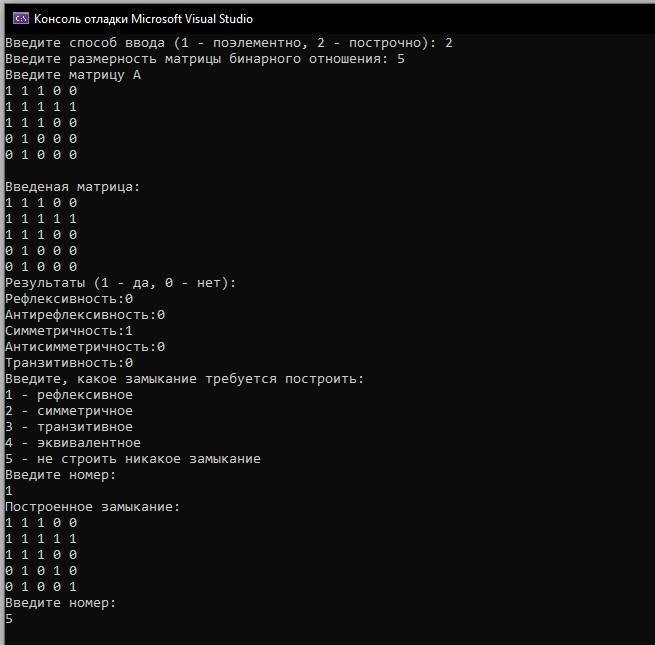
\includegraphics[width=0.9\textwidth]{test1}
		\caption{Тестировние №1}
		\label{fig:test1}
	\end{figure}
	
	Тестирование №2:
	
	На вход поступает матрица:
	
	\begin{pmatrix}
		0 & 0 & 0 & 0 & 0 \\
		1 & 0 & 0 & 0 & 0 \\
		1 & 1 & 0 & 0 & 0 \\
		1 & 1 & 0 & 0 & 0 \\
		1 & 1 & 1 & 0 & 0 
	\end{pmatrix}
	
	Она обладает свойством антирефлексивности, антисимметричности и транзитивности.
	
	Построим все типы замыканий.
	
	\begin{figure}[H]
		\centering
		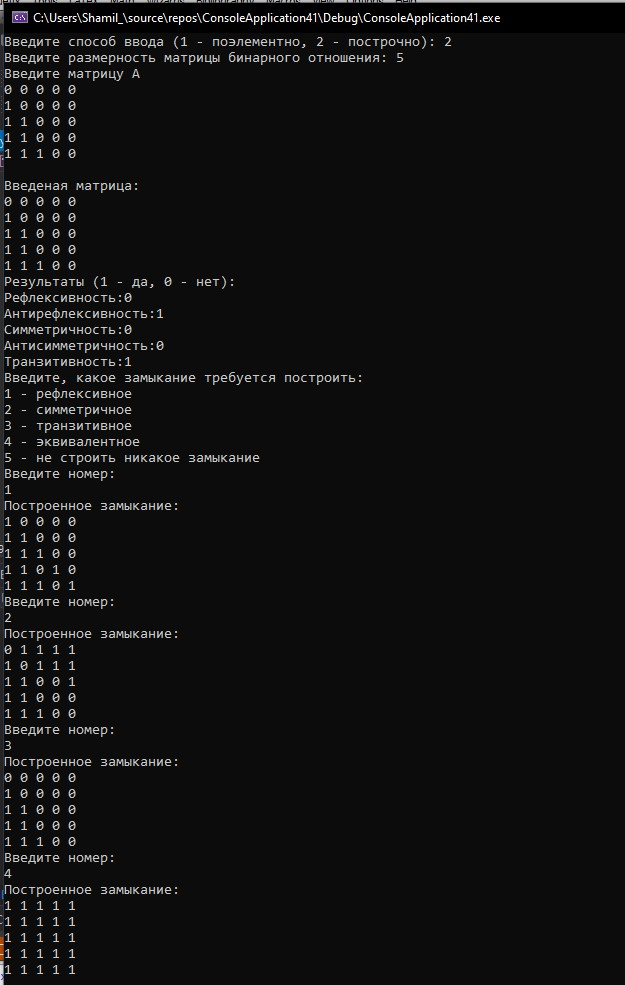
\includegraphics[width=0.9\textwidth]{test2}
		\caption{Тестировние №2}
		\label{fig:test2}
	\end{figure}
	
	Тестирование №3:

	На вход поступает матрица:
	
	\begin{pmatrix}
		1 & 0 & 0 & 0 & 1 \\
		0 & 1 & 1 & 1 & 0 \\
		0 & 1 & 1 & 1 & 0 \\
		0 & 1 & 1 & 1 & 0 \\
		1 & 0 & 0 & 0 & 1 
	\end{pmatrix}
	
	Она обладает свойством рефлексивности, симметричности и транзитивности, а значит является отношением квазипорядка и отношением эквивалентности.

	
	\begin{figure}[H]
		\centering
		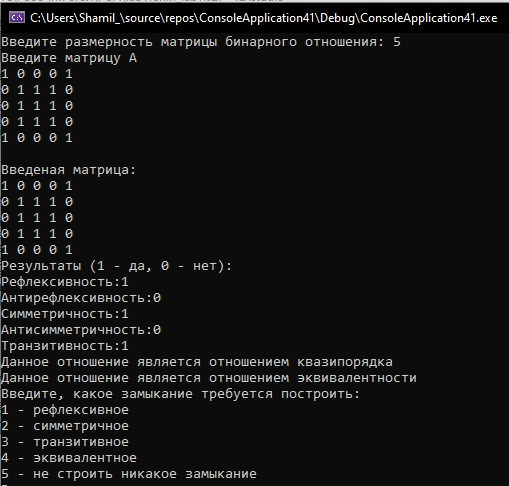
\includegraphics[width=0.9\textwidth]{test3}
		\caption{Тестировние №3}
		\label{fig:test3}
	\end{figure}
	
	\newpage
	\conclusion %заключение
	
	В данной лабораторной работе были рассмотрены и изучены следующие темы: основные определения видов бинарных отношений, свойства бинарных отношений и основные системы замыкания на множестве бинарных отношений. В третьей части работы были реализованы алгоритмы классификации бинарных отношений и построения основных замыканий бинарных отношений.
	
	
\end{document}